\documentclass[11pt]{beamer}
\usetheme{Frankfurt}
\usecolortheme{crane}
\usepackage[utf8]{inputenc}
\usepackage[english]{babel}
\usepackage{amsmath}
\usepackage{amsfonts}
\usepackage{amssymb}
\usepackage{graphicx}
%\usepackage{circuitikz}
\author{Maximilian Heim}
\title{Return Oriented Programming}
%\setbeamercovered{transparent} 
%\setbeamertemplate{navigation symbols}{} 
\logo{\includegraphics[width=1.5cm]{1200px-Hsas_logo.svg.png}}
\institute{University Albstadt-Sigmaringen} 
\date{\today} 
\subject{Offensive Security Methods}
\begin{document}

\begin{frame}
\titlepage
\end{frame}

\begin{frame}
\tableofcontents
\end{frame}

\section{Introduction}
\subsection{Return Oriented Programming}
\begin{frame}
    \frametitle{What is Return Oriented Programming?}
    \begin{enumerate}
    \item A type of buffer overflow attack
    \item Instead of writing executable code onto the stack we place return addresses onto the stack
    \item These get executed sequentially
    \item Using this technique we can achieve arbitrary code execution in large enough programs
    \end{enumerate}
\end{frame}

\begin{frame}
    \frametitle{How does it work?}
    \begin{enumerate}
        \item We have to find "gadgets" in programs
        \item Gadgets are machine instructions that end on a return or jump
    \end{enumerate}
    \begin{figure}[h]
        \caption{ROP Gadgets}
        \centering
        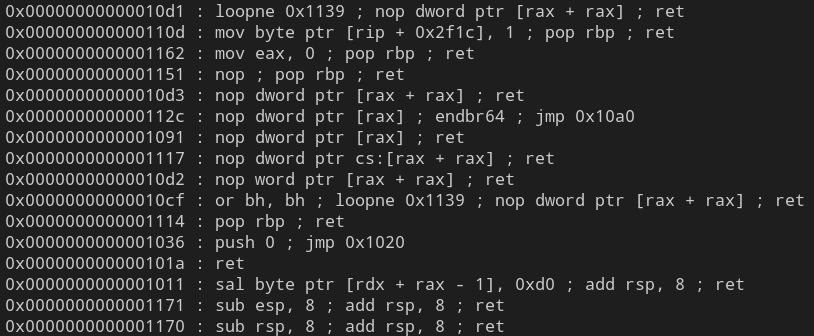
\includegraphics[width=0.9\textwidth]{gadget.png}\label{gadget}
    \end{figure}
\end{frame}
\subsection{Relevanz}
\begin{frame}
    \frametitle{Warum ist es wichtig diese zu erkennen?}
    \begin{itemize}
    \item Militär
    \item Finanzen
    \item Energie
    \item Geheimdienste
    \item Überwachungsstaaten
    \item Transport
    \item U.v.m \ldots
    \end{itemize}

\end{frame}


\section{Erkennung}
\subsection{Destruktive Erkennung}
\begin{frame}
    \frametitle{Reverse Engineering}
    \begin{itemize}
        \item Entfernen der Oberfläche Schicht für Schicht
        \item Advantages: 
        \begin{enumerate}
            \item 100 \% detection rate
        \end{enumerate}
        \item Disadvantages:
        \begin{enumerate}
            \item Only tests a single chip
            \item Chip unusable afterwards
            \item Very time consuming
        \end{enumerate}
        \item However, 
    \end{itemize}
\end{frame}
\subsection{Nicht-Destruktive Erkennung}
\section{Conclusion}
\begin{frame}
    \frametitle{Types of detection}
\end{frame}

\end{document}